\documentclass[aspectratio=43]{beamer}
% Theme works only with a 4:3 aspect ratio
\usetheme{CSCS}

\usepackage{tikz}
\usepackage{pgfplots}
\usepackage{pgfplotstable}
\usetikzlibrary{pgfplots.groupplots,spy,patterns}
\usepackage{listings}
\usepackage{color}
\usepackage{tcolorbox}
\usepackage{anyfontsize}
\usepackage{xspace}
\usepackage{graphicx}

% define footer text
\newcommand{\footlinetext}{Introduction to GPUs in HPC}

% Select the image for the title page
\newcommand{\picturetitle}{cscs_images/image5.pdf}

% fonts for maths
\usefonttheme{professionalfonts}
\usefonttheme{serif}

% source code listing
\newcommand{\axpy}{{\ttfamily axpy}\xspace}

% set indent to a more reasonable level (so that itemize can be used in columns)
\setlength{\leftmargini}{20pt}

\DeclareTextFontCommand{\emph}{\bfseries\color{blue!70!black}}

% Please use the predifined colors:
% cscsred, cscsgrey, cscsgreen, cscsblue, cscsbrown, cscspurple, cscsyellow, cscsblack, cscswhite

\author{Sebastian Keller, Prashanth Kanduri\\ and Ben Cumming, CSCS}
\title{CUDA runtime API and core libraries}
\subtitle{}
\date{\today}

\begin{document}

% TITLE SLIDE
\cscstitle

%%%%%%%%%%%%%%%%%%%%%%%%%%%%%%%%%%%%
\begin{frame}[fragile]{The software ecosystem on top of CUDA}
%%%%%%%%%%%%%%%%%%%%%%%%%%%%%%%%%%%%
    \begin{center}
        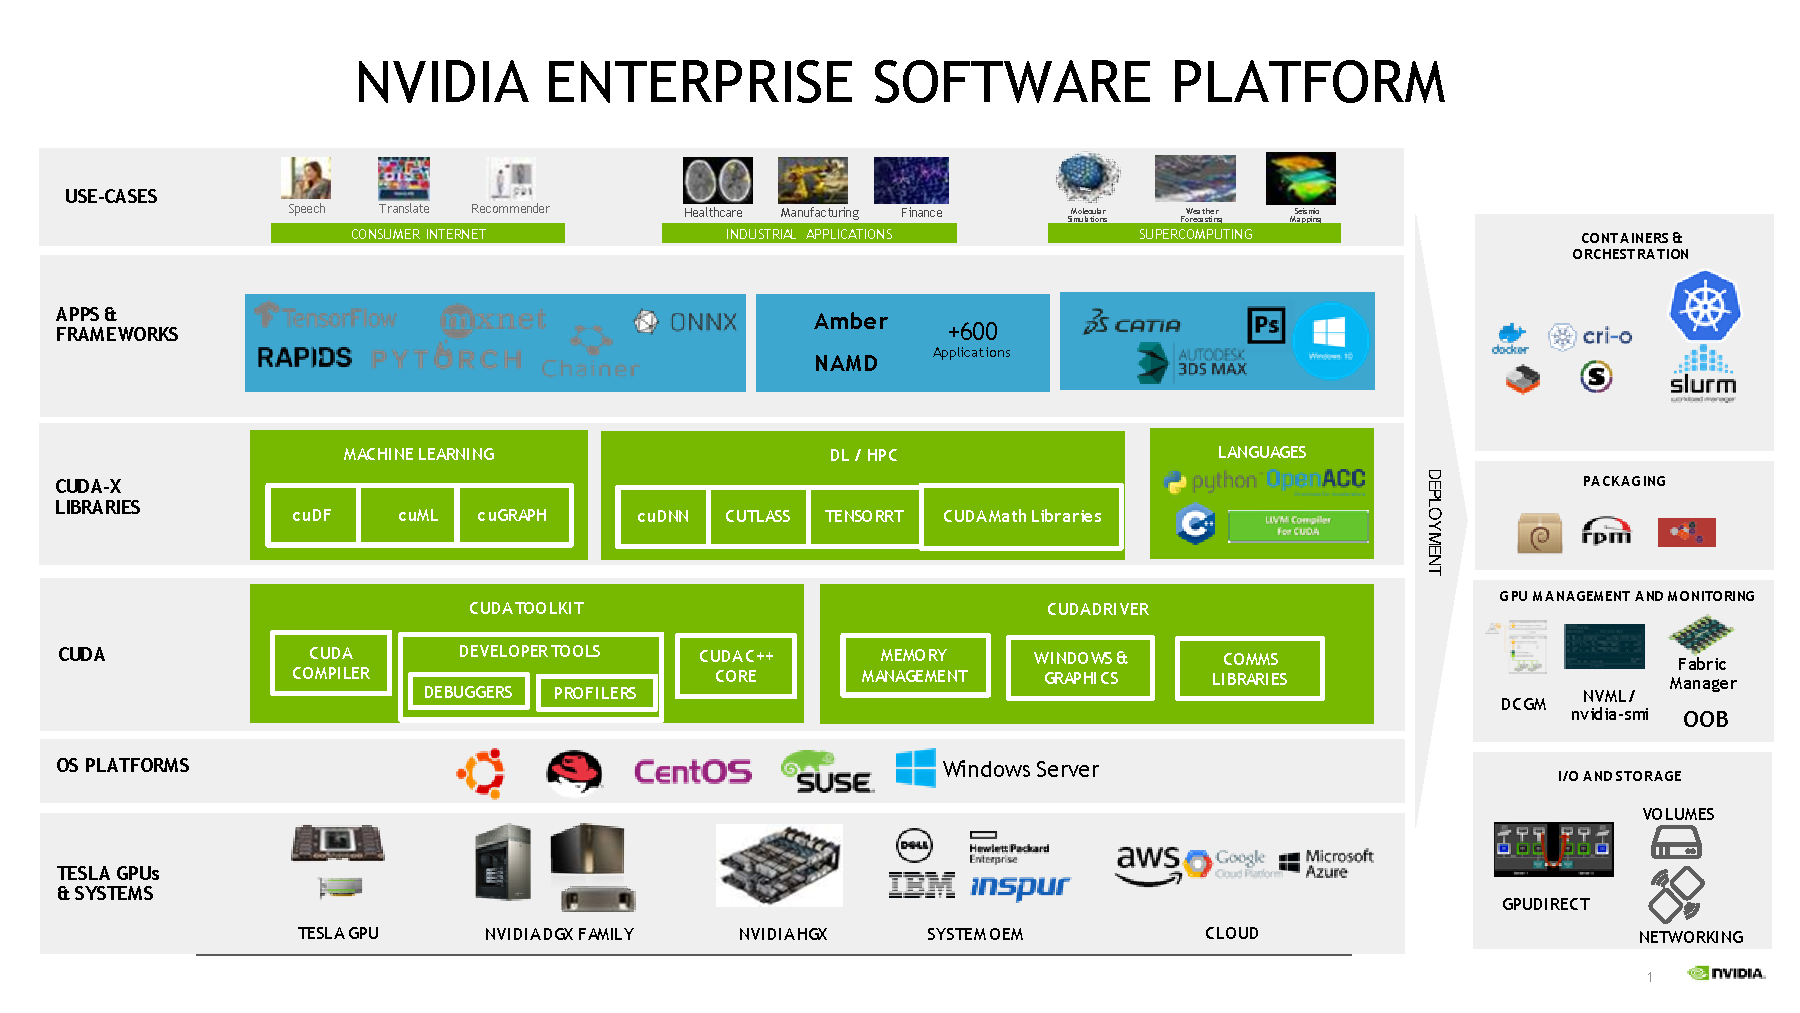
\includegraphics[width=\textwidth]{./images/gpu_platform.pdf}
    \end{center}
\end{frame}

%%%%%%%%%%%%%%%%%%%%%%%%%%%%%%%%%%%%
\begin{frame}[fragile]{The software ecosystem on top of CUDA}
%%%%%%%%%%%%%%%%%%%%%%%%%%%%%%%%%%%%
    \begin{center}
        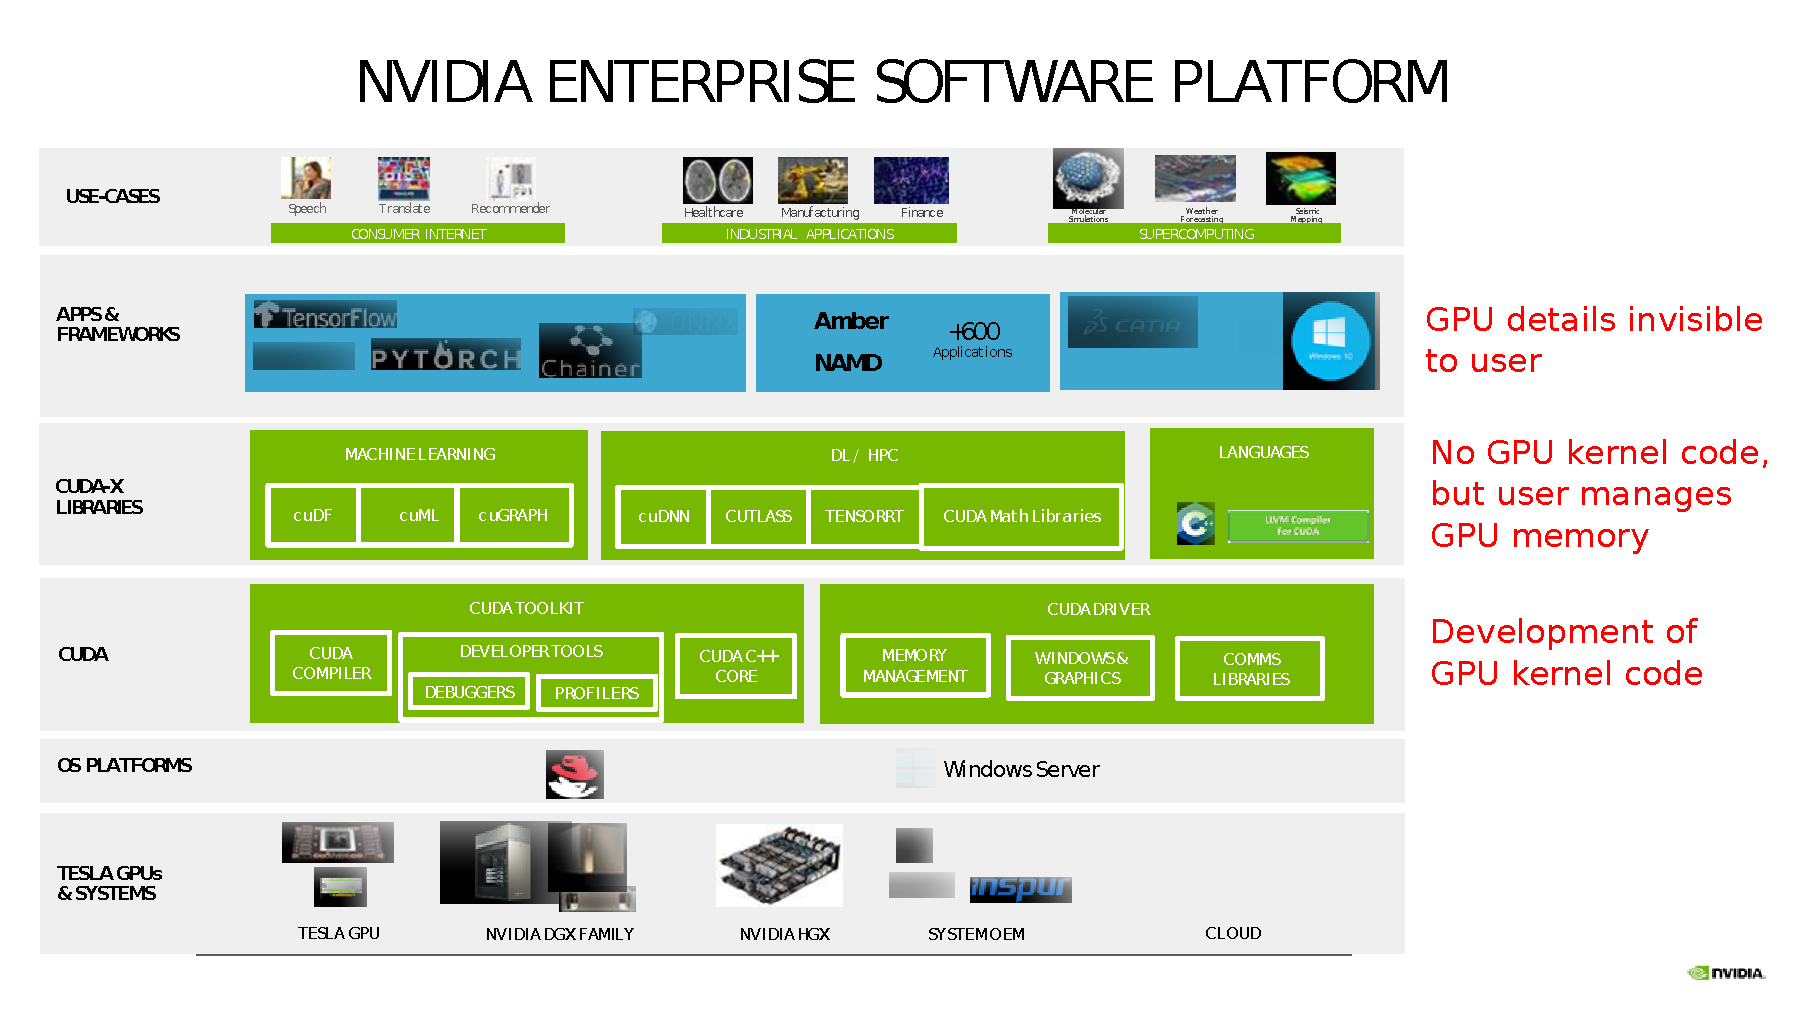
\includegraphics[width=\textwidth]{./images/gpu_layers.pdf}
    \end{center}
\end{frame}

%%%%%%%%%%%%%%%%%%%%%%%%%%%%%%%%%%%%
\begin{frame}[fragile]{Hardware and memory on a Piz Daint Node}
%%%%%%%%%%%%%%%%%%%%%%%%%%%%%%%%%%%%
    \begin{center}
        \includegraphics[width=0.9\textwidth]{./images/node.pdf}
    \end{center}
\end{frame}

%%%%%%%%%%%%%%%%%%%%%%%%%%%%%%%%%%%%
\begin{frame}[fragile]{Hardware and memory on a Piz Daint Node}
%%%%%%%%%%%%%%%%%%%%%%%%%%%%%%%%%%%%
    \begin{center}
        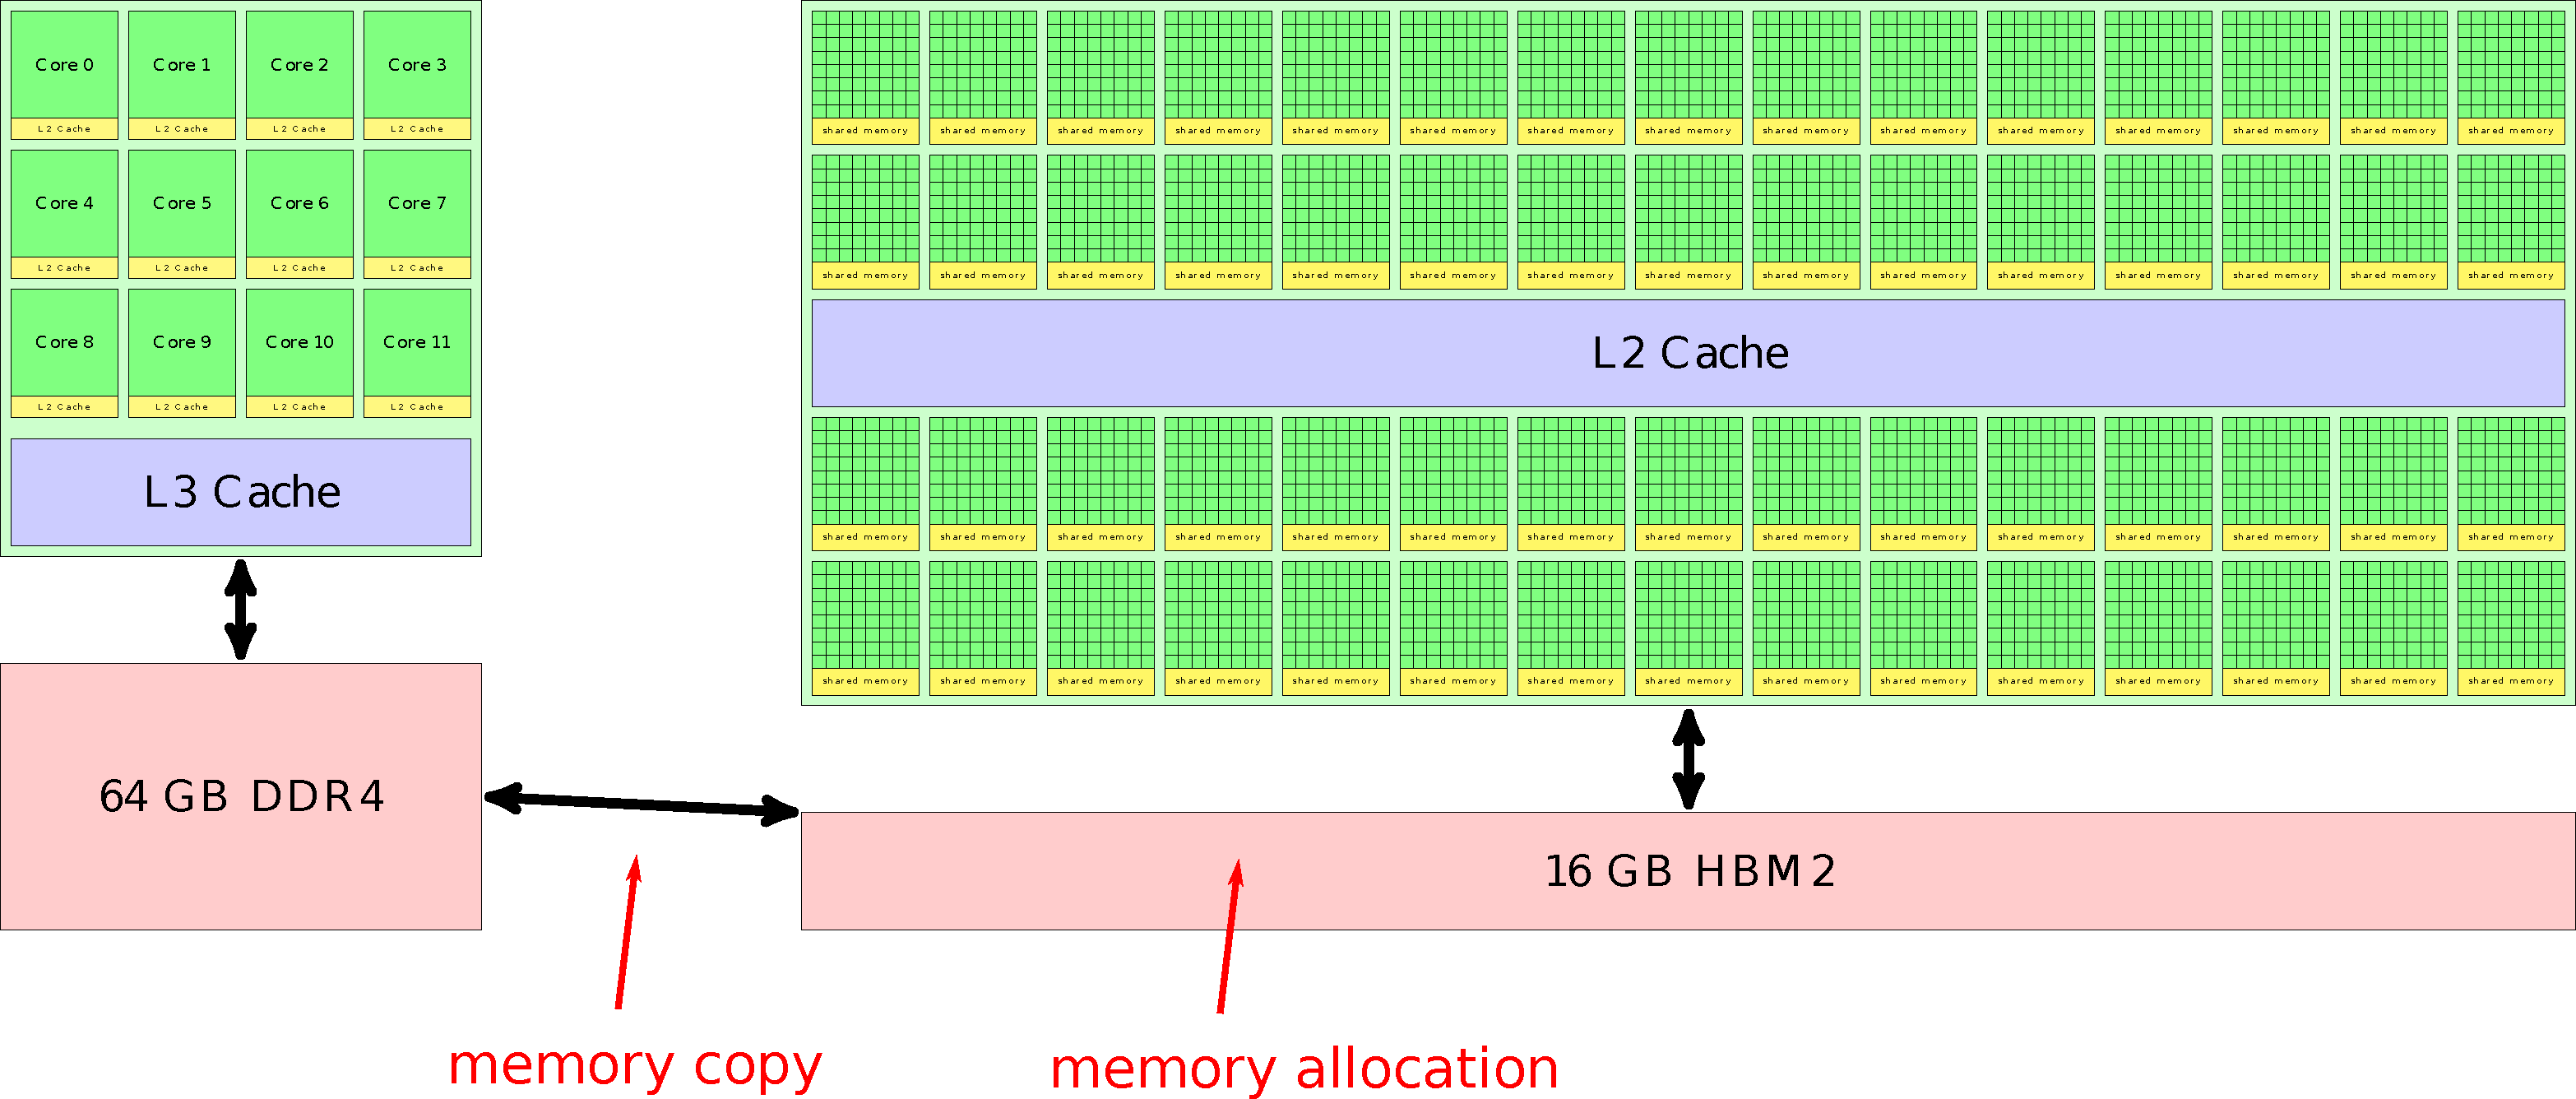
\includegraphics[width=0.9\textwidth]{./images/node_annotated.pdf}
    \end{center}
\end{frame}

%%%%%%%%%%%%%%%%%%%%%%%%%%%%%%%%%%%%
\begin{frame}[fragile]{Host and Device Memory Spaces}
%%%%%%%%%%%%%%%%%%%%%%%%%%%%%%%%%%%%
    \begin{itemize}
        \item The GPU has separate memory to the host CPU
            \begin{itemize}
                \item The host CPU has 64 GB of DDR4 \emph{host memory}
                \item The P100 GPU has 16 GB of HBM2 \emph{device memory}
            \end{itemize}
        \item Kernels executing on the GPU only have fast access to device memory
            \begin{itemize}
                \item Kernel accesses to host memory are copied to GPU memory first over the (slow) PCIe connection.
            \end{itemize}

            \begin{center}
                \begin{tabular}{lcr}
                    \textbf{host $\leftrightarrow$ device} & 11$\times$2 GB/s & PCIe gen3 \\
                    \textbf{host memory}                   & 45 GB/s  & DDR4      \\
                    \textbf{device memory}                 & 558 GB/s & HBM2
                \end{tabular}
            \end{center}

        \item \emph{Optimization tip}: The massive bandwidth of HBM2 on P100 GPUs can only help if data is in the right memory space \emph{before} computation starts.
    \end{itemize}

\end{frame}


%%%%%%%%%%%%%%%%%%%%%%%%%%%%%%%%%%%%
\begin{frame}[fragile]{The CUDA runtime API}
%%%%%%%%%%%%%%%%%%%%%%%%%%%%%%%%%%%%

    %It is possible to allocate host and device memory directly
    \begin{itemize}
        \item Is a \emph{host} library for orchestrating interactions with the device
        \begin{itemize}
            \item allocate memory on the device
            \item copy data between host and device
            \item launch device functions, i.e. kernels
        \end{itemize}
        \item API functions start with \lst{cuda...}
        \begin{itemize}
            \item \lst{cudaMalloc}
            \item \lst{cudaMemcpy}
            \item \lst{<<<...>>>} kernel launch
        \end{itemize}
        \item Calls are made from \emph{CPU} code
    \end{itemize}
\end{frame}


%%%%%%%%%%%%%%%%%%%%%%%%%%%%%%%%%%%%
\begin{frame}[fragile]{Allocating Device Memory with \lst{cudaMalloc}}
%%%%%%%%%%%%%%%%%%%%%%%%%%%%%%%%%%%%

    \begin{itemize}
        \item Can't be read from host
        \begin{itemize}
            \item host has the pointer to device memory
            \item but the host cannot de-reference the pointer 
        \end{itemize}
        \item Need to manually copy data to and from host.
        \item For memory that should always reside on device.
    \end{itemize}
\end{frame}

%%%%%%%%%%%%%%%%%%%%%%%%%%%%%%%%%%%%
\begin{frame}[fragile]{}
%%%%%%%%%%%%%%%%%%%%%%%%%%%%%%%%%%%%
    \begin{info}{Allocating device memory}
        \centering \lst{cudaMalloc(void** ptr, size_t size)}
    \begin{itemize}
        \item \lst{size} number of \emph{bytes} to allocate
        \item \lst{ptr} points to allocated memory on return
    \end{itemize}
    \end{info}

    \begin{info}{Freeing device memory}
        \centering \lst{cudaFree(void* ptr)}
    \end{info}

    \begin{code}{Allocate memory for 100 doubles on device}
%..................................
        \begin{lstlisting}[style=boxcuda]
double* v; // C pointer that will point to device memory
auto bytes = 100*sizeof(double); // size in bytes!
cudaMalloc(&v, bytes); // allocate memory
cudaFree(v);           // free memory
\end{lstlisting}
%..................................
    \end{code}
\end{frame}

%%%%%%%%%%%%%%%%%%%%%%%%%%%%%%%%%%%%
\begin{frame}[fragile]{Copying Memory with \lst{cudaMemcpy}}
%%%%%%%%%%%%%%%%%%%%%%%%%%%%%%%%%%%%

    \begin{itemize}
        \item Accepts device pointers obtained with \lst{cudaMalloc}
        \item Uses the PCI-Express bus to copy between the host and device
        \item Can also be used for copies within the device
    \end{itemize}
\end{frame}

%%%%%%%%%%%%%%%%%%%%%%%%%%%%%%%%%%%%
\begin{frame}[fragile]{}
%%%%%%%%%%%%%%%%%%%%%%%%%%%%%%%%%%%%
    \begin{info}{Perform blocking copy (host waits for copy to finish)}
        \centering \lst{cudaMemcpy(void *dst, void *src, size_t size, cudaMemcpyKind kind)}
    \begin{itemize}
        \item \lst{dst} destination pointer
        \item \lst{src} source pointer
        \item \lst{size} number of \emph{bytes} to copy to \lst{dst}
        \item \lst{kind} enumerated type specifying \emph{direction} of copy:
            \\ one of
            \lst{cudaMemcpyHostToDevice}, \lst{cudaMemcpyDeviceToHost}, \lst{cudaMemcpyDeviceToDevice}, \lst{cudaMemcpyHostToHost}
    \end{itemize}
    \end{info}

    \begin{code}{Copy 100 doubles to device, then back to host}
%..................................
        \begin{lstlisting}[style=boxcuda]
auto size = 100*sizeof(double); // size in bytes
double *v_d;
cudaMalloc(&v_d, size);              // allocate on device
double *v_h = (double*)malloc(size); // allocate on host
cudaMemcpy(v_d, v_h, size, cudaMemcpyHostToDevice);
cudaMemcpy(v_h, v_d, size, cudaMemcpyDeviceToHost);
\end{lstlisting}
%..................................
    \end{code}
\end{frame}

%%%%
\begin{frame}[fragile]{}

    \begin{info}{Errors happen\ldots}
        All API functions return error codes that indicate either:
        \begin{itemize}
            \item success;
            \item an error in the API call;
            \item an error in an earlier asynchronous call.
        \end{itemize}
        The return value is the enum type \lst{cudaError_t}
        \begin{itemize}
            \item e.g. \lst{cudaError_t status = cudaMalloc(&v, 100);}
            \begin{itemize}
                \item status is \{\lst{cudaSuccess}, \lst{cudaErrorMemoryAllocation}\}
            \end{itemize}
        \end{itemize}
    \end{info}

    \begin{info}{Handling errors}
        \centering \lst{const char* cudaGetErrorString(status)}
        \begin{itemize}
            \item returns a string describing status
        \end{itemize}
        \centering \lst{cudaError_t cudaGetLastError()}
        \begin{itemize}
            \item returns the last error
            \item resets status to \lst{cudaSuccess}
        \end{itemize}
    \end{info}

\end{frame}

%%%%
\begin{frame}[fragile]{}

    \begin{code}{Copy 100 doubles to device \emph{with error checking}}
%..................................
        \begin{lstlisting}[style=boxcudatiny]
double *v_d;
auto size = sizeof(double)*100;
double *v_host = (double*)malloc(size);
cudaError_t status;

status = cudaMalloc(&v_d, size);
if(status != cudaSuccess) {
  printf("cuda error : %s\n", cudaGetErrorString(status));
  exit(1);
}

status = cudaMemcpy(v_d, v_h, size, cudaMemcpyHostToDevice);
if(status != cudaSuccess) {
  printf("cuda error : %s\n", cudaGetErrorString(status));
  exit(1);
}
        \end{lstlisting}
%..................................
    \end{code}

    \begin{info}{It is essential to test for errors}
        But it is tedious and obfuscates our source code if it is done in line for every API and kernel call\ldots
    \end{info}
\end{frame}

%%%%%%%%%%%%%%%%%%%%%%%%%%%%%%%%%%%%%%%%%%%%
\begin{frame}[fragile]{Exercise: Device Memory API}
%%%%%%%%%%%%%%%%%%%%%%%%%%%%%%%%%%%%%%%%%%%%
    Open \lst{topics/cuda/practicals/api/util.hpp}
    \begin{enumerate}
        \item what does \lst{cuda_check_status()} do?
        \item look at the template wrappers \lst{malloc_host} \& \lst{malloc_device}
        \begin{itemize}
            \item what do they do?
            \item what are the benefits over using \lst{cudaMalloc} and \lst{free} directly?
            \item do we need corresponding functions for \lst{cudaFree} and \lst{free}?
        \end{itemize}

        \item write a wrapper around \lst{cudaMemcpy} for copying data \texttt{host$\rightarrow$device} \& \texttt{device$\rightarrow$host}
        \begin{itemize}
            \item remember to check for errors!
        \end{itemize}

        \item compile the test and run
        \begin{itemize}
            \item it will pass with no errors on success
        \end{itemize}

    \vspace{-5pt}
\begin{terminal}{}
\begin{lstlisting}[style=terminal]
> make explicit
> srun ./explicit 8
\end{lstlisting}
\end{terminal}
    \end{enumerate}

\end{frame}

%%%%%%%%%%%%%%%%%%%%%%%%%%%%%%%%%%%%%%%%%%%%
\begin{frame}[fragile]{Exercise: Device Memory API}
%%%%%%%%%%%%%%%%%%%%%%%%%%%%%%%%%%%%%%%%%%%%

What does the nvprof profile look like?

\begin{terminal}{}
\begin{lstlisting}[style=terminal]
> srun nvprof -o explicit.nvvp --profile-from-start off -f
    ./explicit 25
> nvvp explicit.nvvp &
\end{lstlisting}
\end{terminal}

\begin{info}{Note about \lst{nvprof}}
For devices newer than the P100, the functionality of \lst{nvprof}
is now offered in two new tools:
  \begin{itemize}
    \item \lst{nsight-sys}
    \item \lst{nsight-compute}.
  \end{itemize}
\end{info}

\end{frame}

%%%%%%%%%%%%%%%%%%%%%%%%%%%%%%%%%%%%
\begin{frame}[fragile]{Using CUDA libraries}
%%%%%%%%%%%%%%%%%%%%%%%%%%%%%%%%%%%%
    \begin{center}
        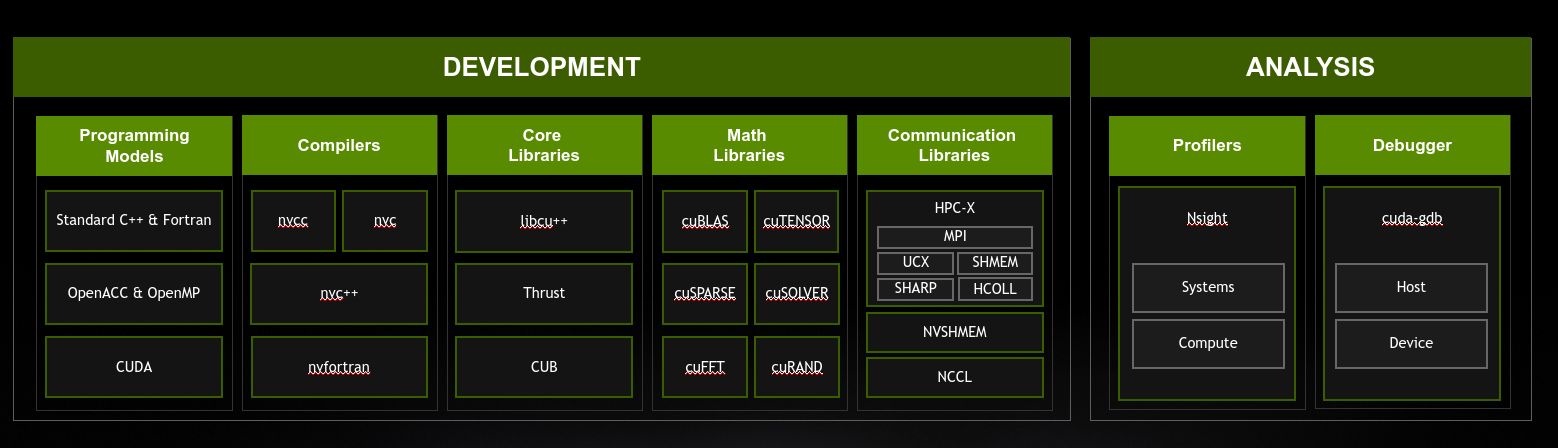
\includegraphics[width=0.9\textwidth]{./image_png/nvidia_libraries.png}
    \end{center}
Managing GPU memory with allocations and data transfers is already enough to
call various GPU libraries, such as:
\begin{itemize}
  \item sorting, reductions, prefix sums
  \item linear algebra and solvers
  \item FFT
  \item etc...
\end{itemize}
\end{frame}


%%%%%%%%%%%%%%%%%%%%%%%%%%%%%%%%%%%%%%%%%%%%
\begin{frame}[fragile]{Some remarks about cuBLAS}
%%%%%%%%%%%%%%%%%%%%%%%%%%%%%%%%%%%%%%%%%%%%

    \begin{code}{excerpt from the cuBLAS example}
%..................................
        \begin{lstlisting}[style=boxcudatiny]
#include <cublas_v2.h>

cublasHandle_t cublas_handle;
cublasCreate(&cublas_handle);

auto cublas_status =
    cublasDaxpy(cublas_handle, n, &alpha, x_device, 1, y_device, 1);

        \end{lstlisting}
%..................................
    \end{code}

    \begin{itemize}
        \item Implements BLAS operations for the device
        \item Compiled library: need an inlude file and link against \lst{-lcublas}
        \item Expects device pointers (from \lst{cudaMalloc})
        \item Data transfer to/from the device is the user's responsiblity
        \item Launched on the host (device-launched version is a separate library)
    \end{itemize}

\end{frame}

%%%%%%%%%%%%%%%%%%%%%%%%%%%%%%%%%%%%%%%%%%%%
\begin{frame}[fragile]{Core libraries: CUB and Thrust}
%%%%%%%%%%%%%%%%%%%%%%%%%%%%%%%%%%%%%%%%%%%%

    \begin{itemize}
        \item CUB (Cuda UnBound) and Thrust are header-only
        \item requires \lst{nvcc} to compile kernel code
        \item CUB
        \begin{itemize}
            \item is CUDA specific
            \item contains header functions for use in device kernel code
            \item contains higher-level operations to launch from host
        \end{itemize}
        \item Thrust
        \begin{itemize}
            \item is platform agnostic
            \item implements algorithms of the C++ STL
            \item CUDA backend built on top of CUB
            \item launched from host
        \end{itemize}
        \item both are built on top of and inter-operable with the CUDA runtime API
    \end{itemize}

\end{frame}

%%%%%%%%%%%%%%%%%%%%%%%%%%%%%%%%%%%%%%%%%%%%
\begin{frame}[fragile]{Some Thrust examples}
%%%%%%%%%%%%%%%%%%%%%%%%%%%%%%%%%%%%%%%%%%%%

    \begin{code}{host and device vectors}
%..................................
        \begin{lstlisting}[style=boxcudatiny]
#include <thrust/host_vector.h>
#include <thrust/device_vector.h>

thrust::device_vector<double> d_vector;
thrust::host_vector<double>   h_vector(10);

// performs cudaMalloc and cudaMempcpy host->device
d_vector = h_vector;

// performs cudaMempcpy device->host
h_vector = d_vector;
        \end{lstlisting}
%..................................
    \end{code}

    \begin{code}{sorting}
%..................................
        \begin{lstlisting}[style=boxcudatiny]
#include <thrust/sort.h>

thrust::sort(thrust::device, d_vector.begin(), d_vector.end());
        \end{lstlisting}
%..................................
    \end{code}

    \begin{code}{reductions}
%..................................
        \begin{lstlisting}[style=boxcudatiny]
#include <thrust/reduce.h>

thrust::reduce(thrust::device, d_vector.begin(), d_vector.end(), 0);
        \end{lstlisting}
%..................................
    \end{code}

\end{frame}

%%%%%%%%%%%%%%%%%%%%%%%%%%%%%%%%%%%%%%%%%%%%
\begin{frame}[fragile]{Thrust interoperability with the runtime API}
%%%%%%%%%%%%%%%%%%%%%%%%%%%%%%%%%%%%%%%%%%%%

    \begin{code}{thrust sort with C-pointers}
        \begin{lstlisting}[style=boxcudatiny]
#include <thrust/device_vector.h>
#include <thrust/sort.h>

double* d_v;
cudaMalloc(&d_v, 100*sizeof(double));

thrust::sort(thrust::device,
             thrust::device_pointer_cast(d_v),
             thrust::device_pointer_cast(d_v + 100));
        \end{lstlisting}
    \end{code}     

\end{frame}

%%%%%%%%%%%%%%%%%%%%%%%%%%%%%%%%%%%%%%%%%%%%
\begin{frame}[fragile]{Exercise: Sorting with Thrust}
%%%%%%%%%%%%%%%%%%%%%%%%%%%%%%%%%%%%%%%%%%%%

    \begin{enumerate}
        \item How does the performance of \lst{std::sort} on the host compare against \lst{thrust::sort}
                on the device?
        \item What if the data transfer times to and from device are included?
    \end{enumerate}
\end{frame}

\end{document}
